
\section{Electron reconstruction and identification}\label{sec:atlas}


The optimal performance in the measurement of electrons and photons plays a fundamental role in searches for new particles, in the measurement of Standard Model cross-sections, and in the precise measurement of the properties of fundamental particles. Here, the electron-based selection is described. Section~\ref{subsec:atlas_detector} describes the ATLAS detector systems in detail with an emphasis on the calorimeter system. The offline electron identification is described in Section~\ref{subsec:electron_offline}. Finally, the electron triggers are described in Section~\ref{subsec:electron_online}.



\subsection{The ATLAS detector}\label{subsec:atlas_detector}

The ATLAS detector is a multipurpose detector designed to observe particles produced in high-energy proton–proton (pp) and heavy-ion (HI) collisions. It is composed of a tracking detector in the innermost region around the interaction point, surrounded by calorimeters and muon chambers. The inner tracking detector (ID) is immersed in a 2 T magnetic field produced by a thin superconducting
solenoid, and provides precise reconstruction of charged-particle tracks in a pseudorapidity\footnote{ATLAS uses a right-handed coordinate system with its origin at the nominal interaction point (IP) in the centre of the detector and the $z$-axis along the beam-pipe. The $x$-axis points from the IP to the centre of the LHC ring, and the $y$-axis points upward. Cylindrical coordinates ($r$, $\phi$) are used in the transverse plane, \phi being the azimuthal angle around the beam-pipe. The pseudorapidity is defined in terms of the polar angle $\theta$ as $\eta = -\ln{\tan(\theta/2)}$. The angular distance $\Delta R$ is defined as $\Delta R = \sqrt{(\Delta\eta)^{2} + (\Delta\phi)^{2}}$ . Transverse momenta and energies are defined as $\pT = p\sin\theta$ and $\ET = E\sin\theta$, respectively.} range $|\eta|<2.47$. The innermost part consists of a silicon pixel detector. A silicon microstrip tracker surrounds the pixel detector with typically four layers of sensor modules. The outermost region of the tracker is covered by a transition radiation tracker (TRT).

The ATLAS calorimeters comprise rectangular cells in the
\etaphi plane for different layers in depth, except for the forward calorimeters. The calorimeter system covers the pseudorapidity range \(|\eta| < 4.9\)~\cite{PERF-2007-01}. Within the region $|\eta|< 3.2$, electromagnetic calorimetry is provided by a high-granularity lead/liquid-argon (LAr) calorimeter (ECal) composed of barrel (EMB1,2,3) sections covering $|\eta|<1.475$ and endcap (EMEC1,2,3) sections covering $1.375<|\eta|<3.2$, with an additional thin LAr presampler (\ps) covering the barrel (PreSamplerB) and endcap (PreSamplerE) regions to correct for energy losses in upstream material~\cite{LARG-2009-01,larg_tdr}. Hadronic calorimetry within $|\eta|< 3.2$ is provided by a steel/scintillator-tile calorimeter (\tilecal)~\cite{TCAL-2017-01,tile_tdr} composed of three barrel sections (TileBar0,1,2) covering $|\eta| < 1.0$ and three extended barrel sections (TileExt1,2,3) covering $0.8<|\eta|< 1.7$, and two copper/LAr hadronic endcap calorimeters (HEC)~\cite{cal_tdr} divided into four modules (HEC0,1,2,3) covering $1.5<|\eta|< 3.2$. Transition regions between calorimeters are used as locations for detector services and induce shower-sharing between calorimeters, which degrades energy measurements in those regions. Here, the barrel-to-endcap transition is complemented by the intermediate tile calorimeter (ITC), which is composed of two modules (TileGap1,2,3) that are attached to the external faces of the barrel and are used to estimate signal losses~\cite{cal_tdr}. The solid-angle coverage is completed with forward
copper/LAr and tungsten/LAr calorimeter (FCal) modules optimized for electromagnetic (EM) and hadronic (HAD) measurements, respectively. The calorimeter system
provides full azimuthal ($\phi$) coverage with a total of about 190\,000 readout cells. 



The electromagnetic and hadronic calorimeters are segmented~\cite{PERF-2007-01} longitudinally (i.e.\ in depth) into three\footnote{The two central layers of each hadronic endcap calorimeter are summed to provide a single measurement.} sampling layers, where each layer has its own lateral ($\eta\times\phi$) granularity. The amount of material in front of each sampling layer varies with \abseta, leading to variations in the expected lateral and longitudinal shower profiles. The expected profiles also depend on the physics object's total energy. In the EM calorimeter, most of the EM shower energy is collected in the second layer (EM2), while the third layer (EM3) provides measurements of energy deposited by the shower tails. However, it should be noted that the first EM layer (EM1) plays an important role in discriminating between photons and $\pi^0$ mesons. The hadronic calorimeters, which surround the EM detectors, provide additional electron discrimination power through energy measurements of possible EM shower tails, as well as rejection of events with activity of hadronic origin via the three sampling layers (HAD1,2,3). The outermost layers of ATLAS consist of an external muon spectrometer (MS) in the pseudorapidity range $|eta|<2.7$. 


\subsection{Offline object reconstruction and identification}\label{subsec:electron_offline}

The offline electron reconstruction uses dynamic, variable-size clusters of energy deposits measured in topologically connected EM and hadronic calorimeter cells [32]. After applying initial position corrections and energy calibrations, they are matched to ID (Inner Detector) tracks re-fitted to account for bremsstrahlung, following the procedure described in [33], to reconstruct electron candidates. 

Prompt electrons entering the central region of the detector ($|\eta|<2.47$) are selected using a likelihood-based (LH) identification [31], which exploits the characteristic features of energy deposits in the EM calorimeters (longitudinal and lateral shower shapes), track quality, track–cluster matching, and particle identification by the transition radiation tracker (TRT). The LH probability density functions (pdfs) for the $E_T$ range of 4.5 to 15 GeV are derived from $J/\Psi\rightarrow ee$ and for $E_T >$ 15 GeV from $Z\rightarrow ee$ events as described in [31]. Different pdfs are obtained for each identification quantity in separate bins in electron-candidate $E_T$ and $\eta$. To ensure a smooth variation of the electron identification efficiency with the electron $E_T$ , the discriminant requirements are varied in $E_T$ finer bins than those defined for the pdfs and, at the $E_T$ bin boundaries, a linear interpolation between the $E_T$ neighboring bins in $E_T$ is used to determine both the pdf values and the discriminant requirements at the $E_T$ bin boundaries. The discriminant threshold is also adjusted linearly as a function of the number of reconstructed vertices to yield a stable rejection of background electrons. Three operating points of electron identification with decreasing efficiency are defined requesting the LH electron ID discriminant of a candidate to be higher than an increasing threshold giving rise to decreasing electron identification efficiencies: ‘Loose’ (93\%), ‘Medium’(88\%) and ‘Tight’(80\%)~\cite{TRIG-2018-01} where the quoted signal efficiencies are computed using electrons produced by electroweak processes integrated over 2015–2017 datasets.

\subsection{Trigger reconstruction and identification}\label{subsec:electron_online}

Electron reconstruction at the HLT stage is performed on each EM RoI provided by L1, which satisfies $E_T$ and isolation requirements as specified by the trigger configuration. It proceeds in a series of sequential steps as shown in the schematic diagram in Figure~\ref{fig:electron_chain}. The hypothesis-test (rectangles) and feature extraction (lozenges) algorithms play a crucial role in the HLT system, where the feature extraction algorithm is responsible for extracting electron characteristics from the detector raw data, such as its energy and impact position in the calorimeter, while the hypothesis-test algorithm uses these attributes to decide if the incoming particle is an electron or a jet.


By combining the output of both, the HLT system can efficiently select events that are likely to be interest for further analysis, while rejecting those that are less relevant. 

\begin{figure}[h!tb]
  \centering
  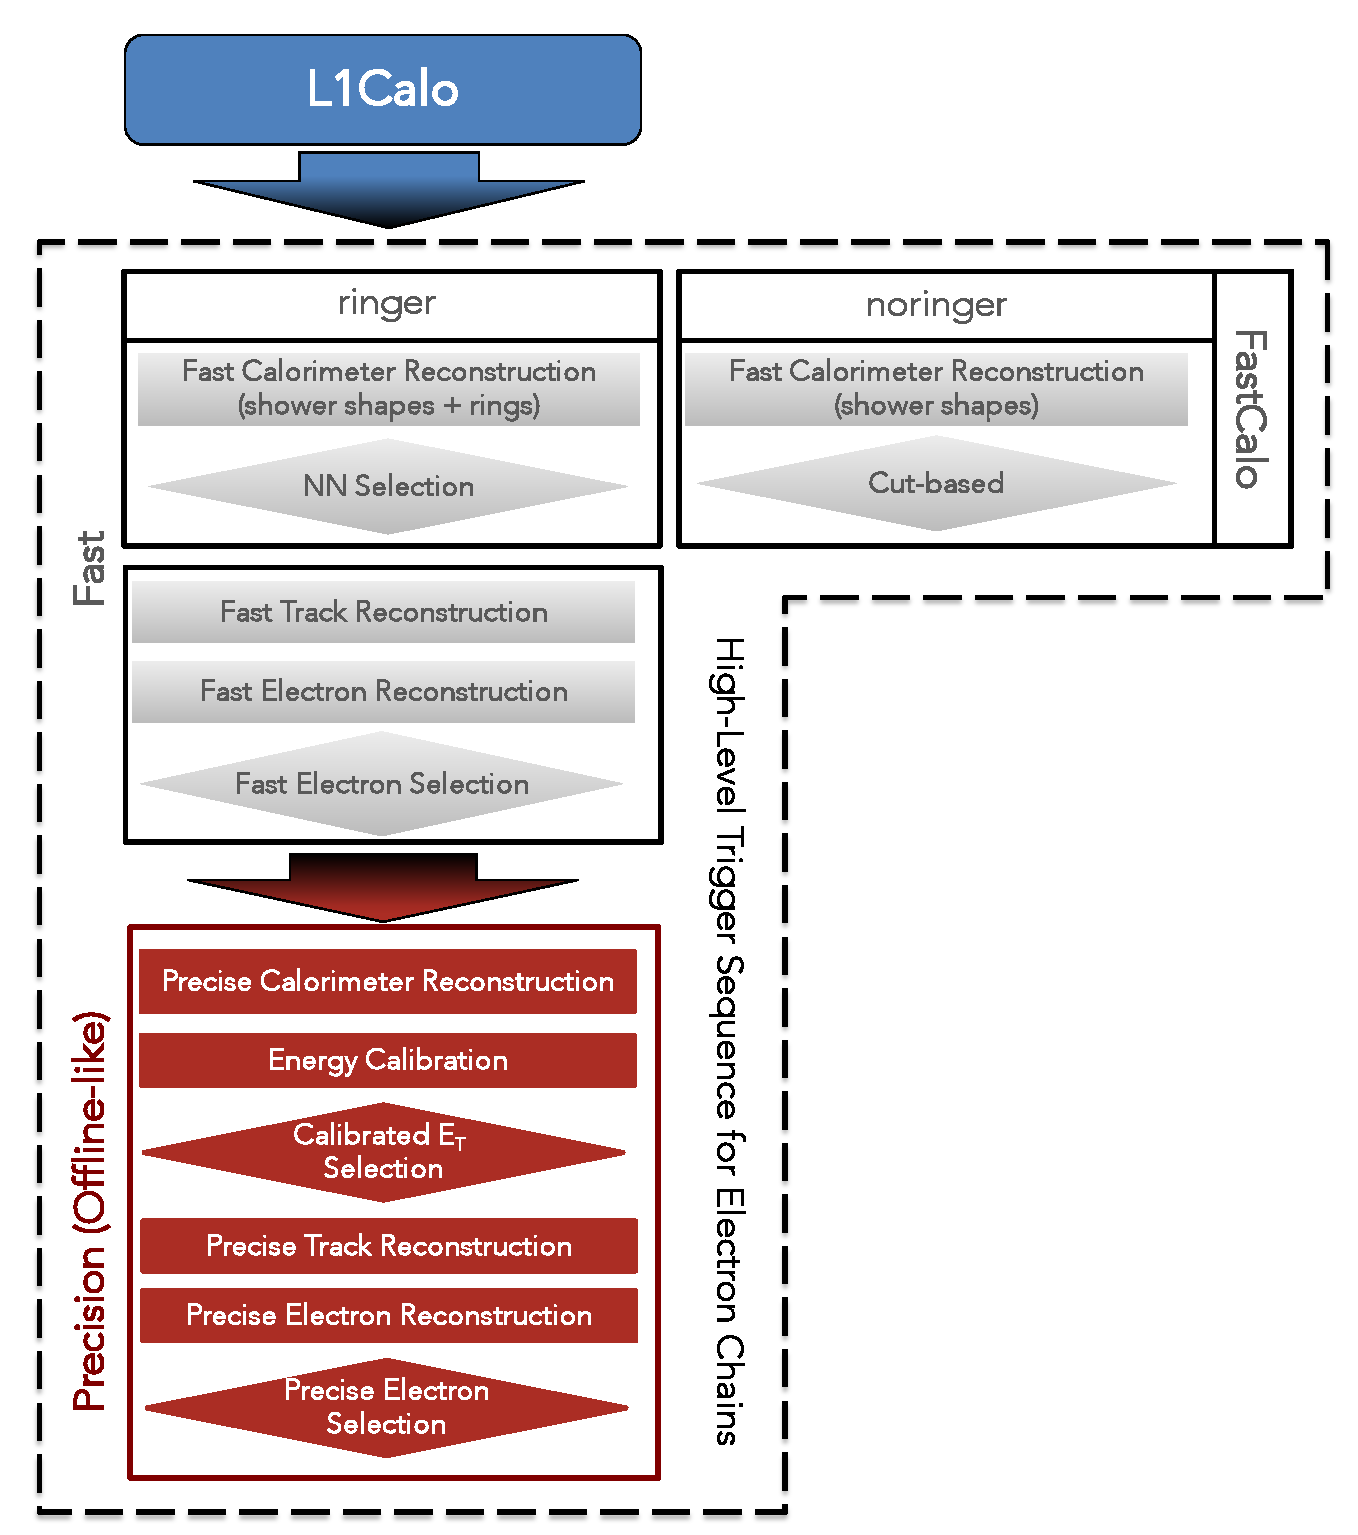
\includegraphics[width=0.7\textwidth]{sections/02_trigger/figures/ElectronChain_Run2_noringer_and_ringer.pdf}
  \caption{This figure presents the  sequence of algorithms used to select electron candidates at the High Level Trigger stage. Differences between the original baseline (no-ringer) and new (ringer) electron triggers lie in the first step, called FastCalo. Grey blocks represent algorithms in the fast stage, and red blocks represent precision-step algorithms.}
  \label{fig:electron_chain}
\end{figure}

In the HLT, fast algorithms are executed first, allowing precision algorithms (which closely reproduce the offline reconstruction algorithms and require more CPU time) to run at a reduced rate later in the trigger sequence. Electron selection starts with a fast calorimeter-reconstruction (FastCalo) step, which has two implementations: the original cut-based selection and the new neural-network (NN) approach using the Neural-Ringer algorithm presented in this paper. This is followed by a fast track-reconstruction step, which also places requirements on variables that indicate the quality of proximity matching between the electron candidate positions reconstructed from the track and the calorimetric measurements. If a particle candidate satisfies the criteria defined for the fast electron selection, the precision algorithms are executed in the HLT, where access to detector information outside the RoI is possible. These precision online algorithms are similar to their offline counterparts. 
The precision electron selection relies on a multivariate technique using a LH discriminant with four operating points: ‘lhvloose’, ‘lhloose’, ‘lhmedium’, and ‘lhtight’. The identification in the trigger is designed to be as close as possible to the offline version, but there are a few necessary differences: the discriminating variables used online have different resolutions; the online selection uses \avgmu{} to assess pileup\footnote{an overlap of multiple proton-proton collisions within the detector, resulting in a superposition of particle signals in the same LHC bunch-crossing.} and adjust the discriminant threshold requirement, while the number of primary vertices is used offline; some discriminating variables used in offline selection are not present in online version due to CPU constraints.

Triggers with ‘nod0’ suffixed to their names do not include the transverse impact parameter relative to the beam-line, $d_0$, and its significance, in the online LH version. An additional, optional requirement of isolation denoted ‘ivarloose’ is also available for electron triggers. This tracking-only isolation is required to satisfy 
$p_T^{iso}(\Delta R^{var}<0.2)/p_T < 0.10$ and is calculated similarly to the offline isolation operating points.
